\chapter{Bringing pieces together: the biological role of IL-10-GAG interaction}
\label{together}
%\markboth{Bringing pieces together: the biological role of IL-10-GAG interaction}%
%{Bringing pieces together: the biological role of IL-10-GAG interaction}

In this short chapter, I assemble important insights about the IL-10-GAG system
derived in this thesis and try to bring them into the biological context. Some
of these insights have a synergy effect, i.e.\ they support each other and
provide rather strong clues about how the IL-10-GAG system may behave in nature
on the molecular level.


\subsubsection{Experimental input: non-random, but weak interaction}

As noted in \cref{chapter:nmr}, our collaborators in Prof. Huster's NMR
laboratory at the Universität Leipzig could confirm binding between heparin
oligosaccharides and murine IL-10. As of the high similarity between human and
murine IL-10 (see \cref{background:il10biologyprimer}), this result is very
likely transferable between species. As published \cite{kuenze_gehrcke_2014},
the binding affinity between IL-10 and HP oligosaccharides measured in G.
Künze's NMR essays was determined to be in the micromolar range, whereas
Salek-Ardakini et al.\ found a binding affinity in the nanomolar range
\cite{salek_ardakani_2000}. Considering the differences in the investigated
systems (polymeric HP \textit{versus} oligomeric HP, human IL-10 \textit{versus}
murine IL-10) and the entirely different experimental techniques, it is no
worrying contradiction that both results differ by an order of magnitude.

The experimentally obtained binding affinity results and the observation that
IL-10-HP interaction has a measurable impact on the backbone structure of HP
(see \cref{chapter:nmr}) are strong indications that IL-10 and HP interact in a
non-random fashion. However, various indicators point towards a rather weak
interaction, compared to e.g.\ FGF2-HP. One of these pointers is that HP dp4's
iduronic acid populates both, the ${}^1$C${}_4$ and ${}^2$S${}_\mathrm{O}$
conformations in the bound state (see \cref{chapter:nmr}).


\subsubsection{Putative binding poses fit experimental data}

In \cref{chapter:bspred}, a putative IL-10-GAG binding region (occurring twice
as of the symmetry of the IL-10 homodimer) has been proposed, based on the
analysis of IL-10's Coulomb potential. In \cref{chapter:dmdil10}, it is
described how this binding region was further analyzed with DMD, and narrowed
down towards single key amino acids (being most responsible for GAG binding) and
towards two principal putative GAG binding poses, named A and B (see
\cref{fig:dmdil10:2nd_stage_principal_poses}). These poses are in close
proximity to R107, which has been identified as especially important for GAG
binding, and have special relations to experimentally obtained data, as will be
described in the following paragraphs.

\begin{figure}
\centering
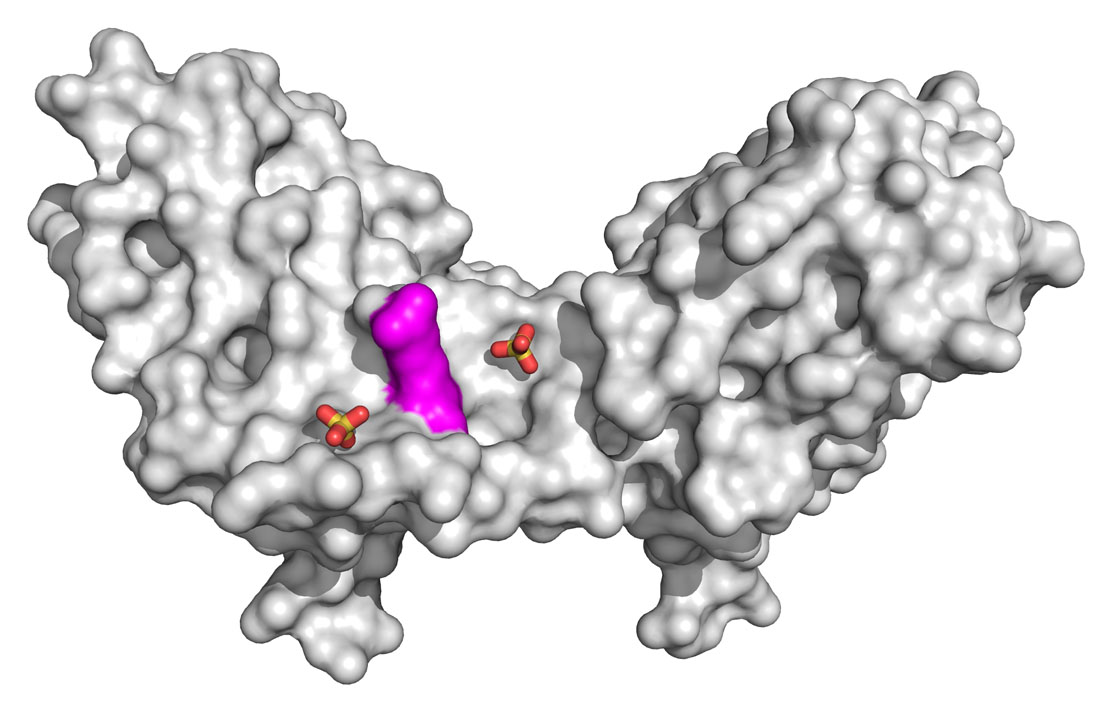
\includegraphics[width=1.0\textwidth]{gfx/together/il10sulfates_01.jpg}
\caption[]{
Structure of human IL-10 according to PDB entry 2ILK in surface representation,
including two sulfate groups contained in the crystal structure, shown in thick
stick representation. The surface of IL-10's amino acid residue R107 is colored
in magenta. During crystal growth, sulfate groups assume energetically favorable
positions, which are transferable to sulfate groups in GAGs.}
\label{fig:together:il10sulfates}
\end{figure}

In protein crystallization, sulfates are often used for diminishing the
electrostatic repulsion and for promoting the hydrophobic interactions among
proteins and therefore for facilitating crystal growth
\cite{crystal_salts_2001}. In high-quality crystal structures, the atomic groups
of these sulfates are spatially resolved and visible. Obviously, during crystal
growth, these atomic groups end up in positions that are physically favorable
for them and therefore provide valuable input when it comes to the investigation
of protein-GAG interaction: it is valid to assume that the very same locations
would also be energetically favorable for sulfate groups contained in GAGs.

Three sulfate groups are contained in the 2ILK crystal structure of IL-10 (which
has been used throughout this thesis). Two of these sulfate groups are located
right in the neighborhood of R107, as shown in \cref{fig:together:il10sulfates}.
The location of the sulfate groups contained in the 2ILK crystal structure is a
strong experimental support of the putative IL-10-GAG binding region proposed in
\cref{chapter:bspred}. Furthermore, the imaginary line connecting both sulfate
groups aligns well with one of the two putative GAG binding poses proposed in
\cref{dmdil10:2ndstageresults} (pose A, see
\cref{fig:dmdil10:2nd_stage_principal_poses}). The putative GAG binding pose B
crosses the position of one of both sulfate groups.

As described in \cref{chapter:nmr}, NMR data suggests a cooperative binding mode
in which a GAG oligosaccharide bridges both symmetrically aligned putative
IL-10-GAG binding regions. In a thought experiment, extended versions of both
putative GAG binding poses, A and B, can be imagined to connect both binding
regions on the front and back of the IL-10 V-shape. For binding mode B, however,
this seems to be a more probable scenario than for binding mode A.


\subsubsection{Scenario: modulation of IL-10 biology by impaired diffusion}

\begin{figure}
\centering
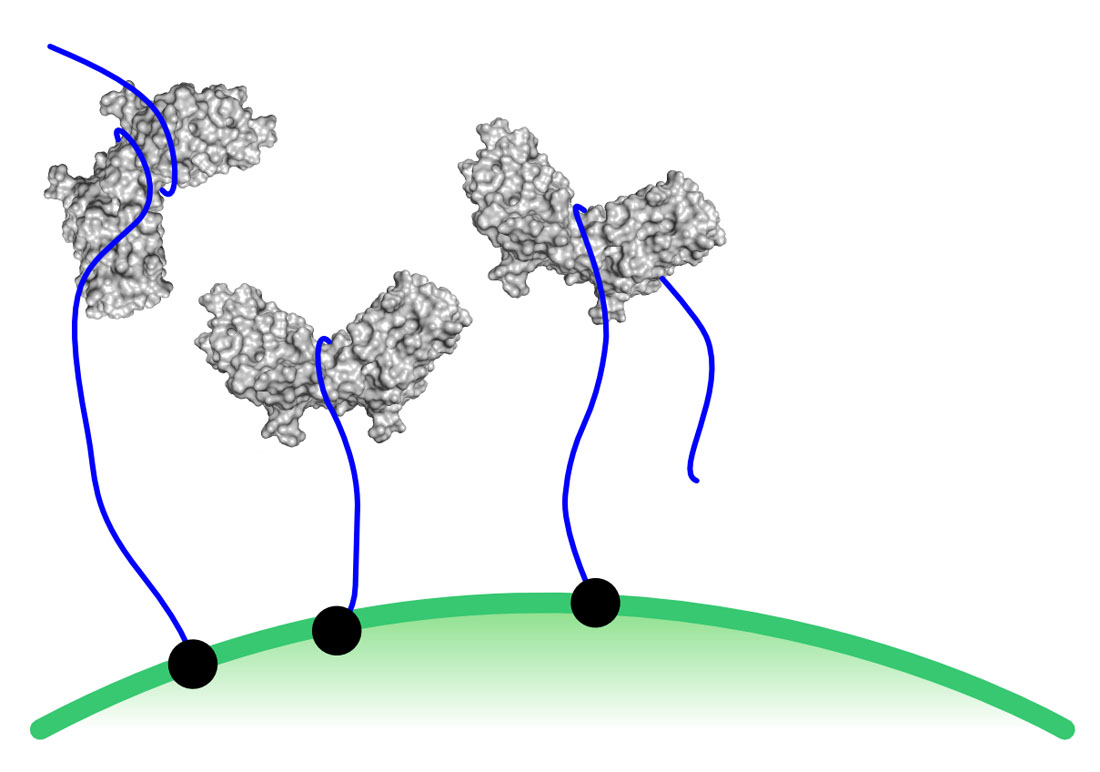
\includegraphics[width=1.0\textwidth]{gfx/together/agglomeration_small.jpg}
\caption[]{
Conceptual visualization of how cell surface-attached proteoglycans (black) with
long GAG chains (blue) might impair IL-10 (gray) diffusion. The cell membrane is
here indicated in green, with the inner part of the cell being at the bottom.
Size ratios and the exact location and curvature of the GAG polysaccharides are
not to be taken literally.}
\label{fig:together:diffusionimpaired}
\end{figure}

In literature it is often speculated that cytokine-GAG interaction for certain
systems does not directly affect the signaling cascade, but rather may be a
mechanism for cytokine concentration and diffusion control, e.g.\ for retaining
a type of cytokine close to its site of secretion in the tissue (see
\cref{background}). After the findings made in this thesis project, the scenario
in which longer GAG chains impair the diffusion of IL-10 without affecting the
IL-10 receptor system seems to be a valid model.

Considering the IL-10 ternary complex model discussed in
\cref{background:structureil10system} and shown in
\cref{fig:bg:il10_il10r1_il10r2_model}, the interaction of IL-10 with its
receptors is focused towards the sides of IL-10's V-shape. The IL-10-GAG
interaction, however, is predicted to mainly occur in the groove of the V-shape,
especially regarding a potential cooperativeness of both symmetrically aligned
binding regions. It is therefore entirely conceivable that IL-10-GAG interaction
may \textit{not} affect the interaction between IL-10 and both of its
receptors. At the same time, a cooperative \enquote{attack} of a polymeric GAG
chain focused on the groove of the V would be an effective mechanism for
impairing the diffusion of the IL-10 homodimer, assuming that the GAG chain is
fixed on at least one side. This model would very well fit the idea of impaired
cytokine diffusion due to cell surface-attached proteoglycans, as schematically
depicted in \cref{fig:together:diffusionimpaired}.


\subsubsection{Scenario: modulation of IL-10 biology by interference with
receptor binding}

While the above-presented scenario of a GAG-induced impaired IL-10 diffusion
fits the findings obtained in this thesis project quite well, a more direct
impact of GAG molecules on IL-10 biology via involvement in receptor binding can
not be excluded. Specifically, in the ternary IL-10 complex binding model
(discussed in \cref{background:structureil10system} and shown in
\cref{fig:bg:il10_il10r1_il10r2_model}), IL-10R2 has contacts to IL-10 that are
potentially quite close to R107, see \cref{fig:together:r2impaired}. In this
model, it is conceivable that a GAG molecule bound in close proximity to R107
could sterically impede formation of the ternary complex required for IL-10
signaling. The GAG molecule would therefore have a direct impact on the
biological activity of IL-10. It should be stressed that this scenario is
speculative but allowed in the framework of the information obtained about the
IL-10-GAG system so far. Specifically, according to this model, a GAG bound in
the principal binding mode A shown in
\cref{fig:dmdil10:2nd_stage_principal_poses} would interfere with IL-10R2. On
the other hand, it should be noted that no solid data has been obtained in the
course of this project that suggest that GAGs could interfere with the
interaction between IL-10 and IL-10R1.

\begin{figure}
\centering
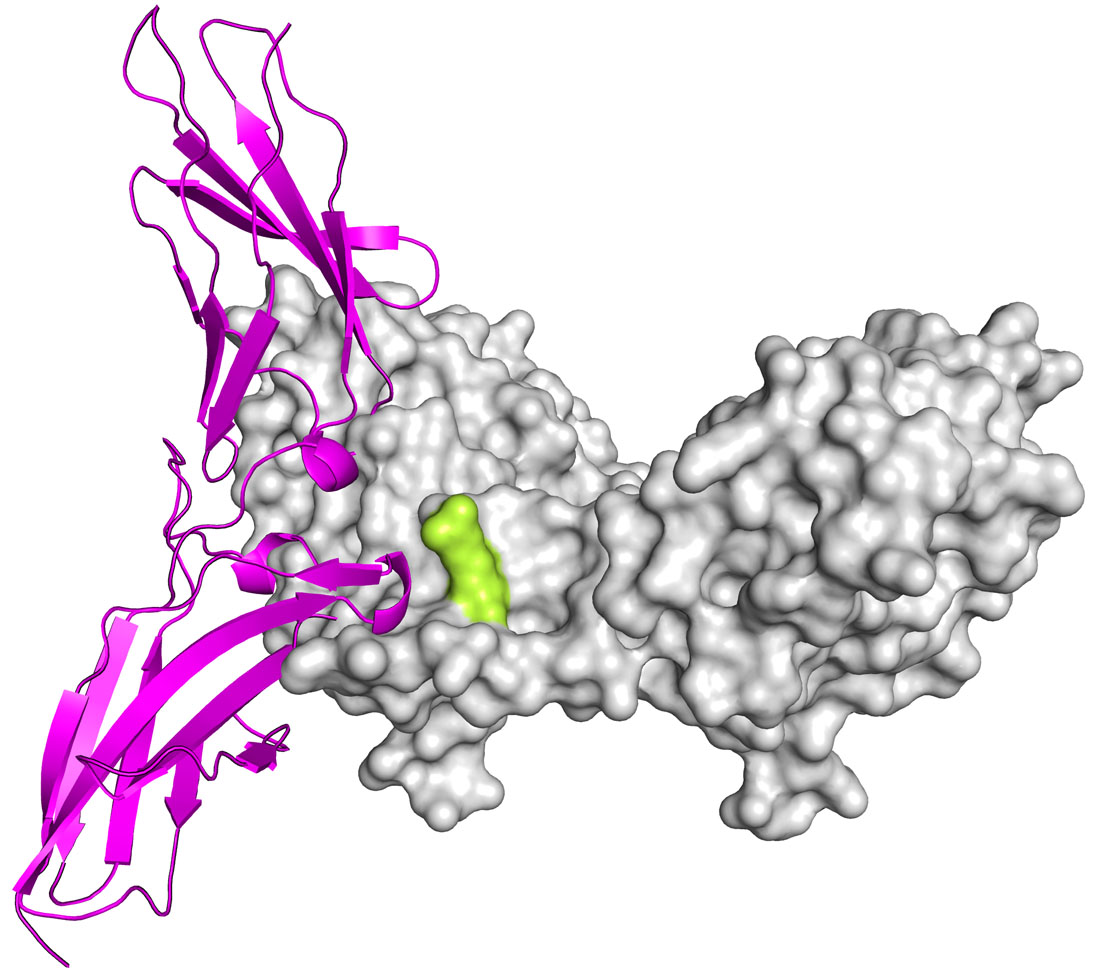
\includegraphics[width=1.0\textwidth]{gfx/together/il10dimer_surface_r2cartoon_r107_01.jpg}
\caption[]{
Binding model of IL-10R2 (magenta) and IL-10 (gray) as previously described in
\cref{background:structureil10system}, with R107 highlighted in yellow. Here,
the close proximity between R107 to IL-10R2 is to be pointed out, which suggests
a potential structural interference between a GAG molecule bound near R107 on
the one hand, and IL-10R2 on the other hand.}
\label{fig:together:r2impaired}
\end{figure}
